\section{Experiments}\label{sec:experiments}

\subsection{Evaluation Setup}

\paragraph{Implementation}
All models and experiments are implemented using PyTorch~\citep{Paszke2019PyTorch}.

\paragraph{Model and Dataset}
We employ pretrained VGG16 and ResNet18 models on the ImageNet \cite{Deng2009} classification task.
Because localization metrics require ground-truth object segmentation masks, we evaluate on ImageNet-S-50~\citep{Gao2022imagenets}, which provides pixel-level semantic segmentation annotations for 50 ImageNet classes, excluding unsegmentable classes (\eg \emph{bookshop}).
The reported experiment uses a validation set of 50 images, one randomly selected for each class, and a test set of 566 images. The released loader selects from locally available image--mask pairs and does not check agreement between the annotation class and the official ILSVRC2012 label; the historical sample membership cannot be reconstructed from the reported counts alone. Attributions target the model's predicted class, including for misclassified images, while localization is evaluated against the annotated object mask.

\paragraph{Baseline Methods}
We compare our Split methods against a range of established attribution approaches. Gradient-based methods include Saliency~\citep{Simonyan2014}, Input~$\times$~Gradient~\citep{Shrikumar2017}, Integrated Gradients~\citep{Sundararajan2017} and GradientSHAP~\citep{LundbergLee2017}. CAM-based methods comprise Layer-CAM~\citep{Jiang2021LayerCAM} and Grad-CAM++~\citep{Chattopadhay2018}. Among propagation-based techniques, we evaluate DeepLift~\citep{Shrikumar2017} and standard LRP with $\gamma=0.25$~\citep{Bach2015}. Finally, perturbation-based baselines include Occlusion~\citep{ZeilerFergus2014} and Feature Ablation.
For baseline $\gamma$-LRP comparisons, we use the Zennit library in the default setting~\citep{Anders2021Zennit}.
For all other baselines we use the Captum \citep{kokhlikyan2020captum} implementations in their default settings, except for GradCAM++ and LayerCAM, where we use own implementations.

\newcommand{\colA}{0.10}
\newcommand{\colB}{0.075}
\newcommand{\colSpace}{0.0015\linewidth}

\begin{figure*}[!t]
    \centering

    \begin{minipage}[c]{\colA\linewidth}\centering\scriptsize\textbf{Class}\end{minipage}\hspace{\colSpace}%
    \begin{minipage}[c]{\colB\linewidth}\centering\scriptsize\textbf{Original}\end{minipage}\hspace{\colSpace}%
    \begin{minipage}[c]{\colB\linewidth}\centering\scriptsize\textbf{SplitLRP}\\\scriptsize\textbf{$R^{(10,\text{pos})}$ abs}\end{minipage}\hspace{\colSpace}%
    \begin{minipage}[c]{\colB\linewidth}\centering\scriptsize\textbf{LRP $\gamma$=0.25}\\\scriptsize\textbf{layer 5 abs}\end{minipage}\hspace{\colSpace}%
    \begin{minipage}[c]{\colB\linewidth}\centering\scriptsize\textbf{SplitCAM}\\\scriptsize\textbf{$\alpha=0.4$}\\\scriptsize\textbf{$\delta^{(14,g)}$}\end{minipage}\hspace{\colSpace}%
    \begin{minipage}[c]{\colB\linewidth}\centering\scriptsize\textbf{LayerCAM}\\\scriptsize\textbf{layer 14}\end{minipage}\hspace{\colSpace}%
    \begin{minipage}[c]{\colB\linewidth}\centering\scriptsize\textbf{SplitCAM}\\\scriptsize\textbf{$\alpha=0.3$}\\\scriptsize\textbf{$\delta^{(26,g)}$ abs}\end{minipage}\hspace{\colSpace}%
    \begin{minipage}[c]{\colB\linewidth}\centering\scriptsize\textbf{LayerCAM}\\\scriptsize\textbf{layer 26}\end{minipage}\hspace{\colSpace}%
    \begin{minipage}[c]{\colB\linewidth}\centering\scriptsize\textbf{SplitGrad}\\\scriptsize\textbf{$\alpha=0.3$}\\\scriptsize\textbf{$\delta^{(0,+,g)}$}\end{minipage}

    \vspace{0.25cm}

    \begin{minipage}[c]{\colA\linewidth}
        \centering
        \small goldfinch\\[1pt]
        {\scriptsize (0.9996)}
    \end{minipage}\hspace{\colSpace}%
    \begin{minipage}[c]{\colB\linewidth}
        \centering
        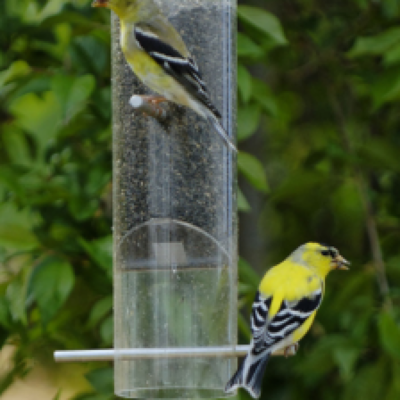
\includegraphics[width=\linewidth]{saliency_quality/image_0030_ILSVRC2012_val_00030071.JPEG/original_image.png}
    \end{minipage}\hspace{\colSpace}%
    \begin{minipage}[c]{\colB\linewidth}
        \centering
        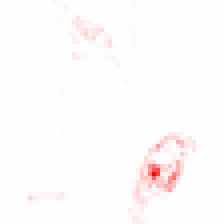
\includegraphics[width=\linewidth]{saliency_quality/image_0030_ILSVRC2012_val_00030071.JPEG/hybrid_lrp_scaling_max_winnerTakesItAllMaxpool_f10_cam_pp_abs.png}
    \end{minipage}\hspace{\colSpace}%
    \begin{minipage}[c]{\colB\linewidth}
        \centering
        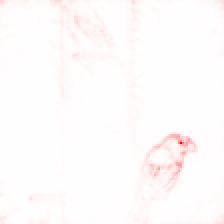
\includegraphics[width=\linewidth]{saliency_quality/image_0030_ILSVRC2012_val_00030071.JPEG/zennit_lrp_gamma0.25_features_5_abs.png}
    \end{minipage}\hspace{\colSpace}%
    \begin{minipage}[c]{\colB\linewidth}
        \centering
        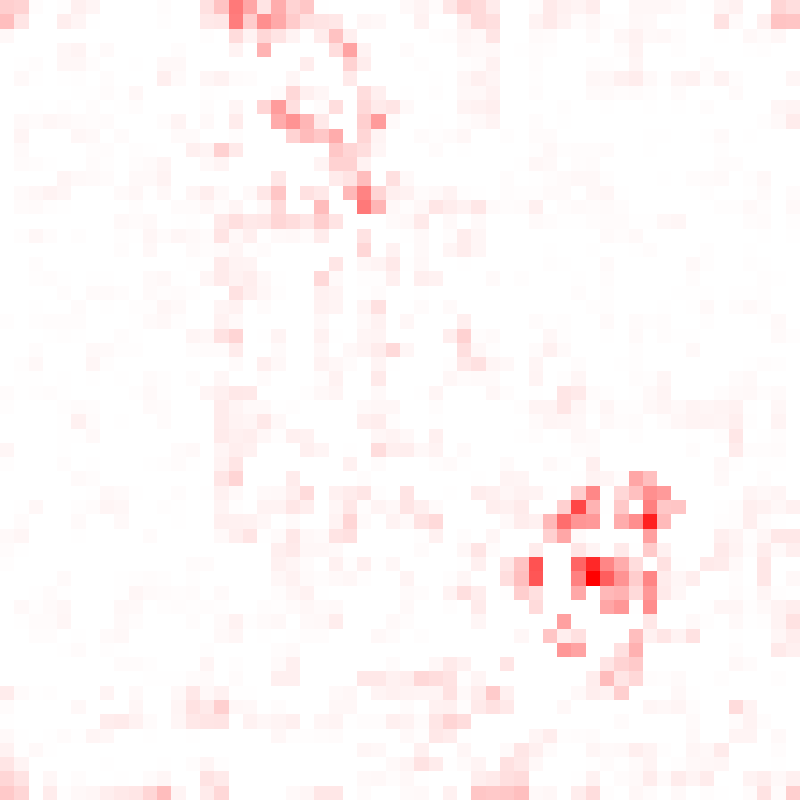
\includegraphics[width=\linewidth]{saliency_quality/image_0030_ILSVRC2012_val_00030071.JPEG/hybrid_cam_shift_40_scale_max_winnerTakesItAllMaxpool_f14_cam_g.png}
    \end{minipage}\hspace{\colSpace}%
    \begin{minipage}[c]{\colB\linewidth}
        \centering
        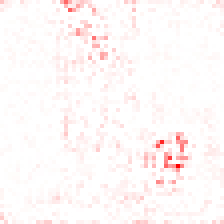
\includegraphics[width=\linewidth]{saliency_quality/image_0030_ILSVRC2012_val_00030071.JPEG/layer_cam_features_14_relu.png}
    \end{minipage}\hspace{\colSpace}%
    \begin{minipage}[c]{\colB\linewidth}
        \centering
        
\includegraphics[width=\linewidth]{saliency_quality/image_0030_ILSVRC2012_val_00030071.JPEG/hybrid_cam_shift_30_scale_max_winnerTakesItAllMaxpool_f26_cam_g_abs.png}
    \end{minipage}\hspace{\colSpace}%
    \begin{minipage}[c]{\colB\linewidth}
        \centering
        
\includegraphics[width=\linewidth]{saliency_quality/image_0030_ILSVRC2012_val_00030071.JPEG/layer_cam_features_26_relu.png}
    \end{minipage}\hspace{\colSpace}%
    \begin{minipage}[c]{\colB\linewidth}
        \centering
        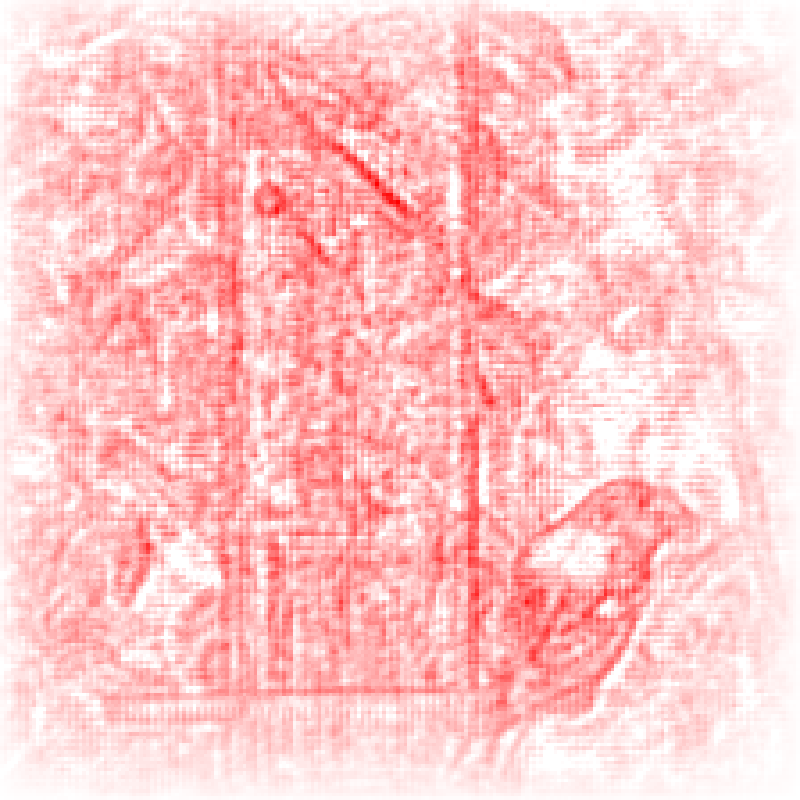
\includegraphics[width=\linewidth]{saliency_quality/image_0030_ILSVRC2012_val_00030071.JPEG/hybrid_grad_shift_30_max_winnerTakesItAllMaxpool_f0_grad_pp.png}
    \end{minipage}%

    \vspace{0.25cm}

    \begin{minipage}[c]{\colA\linewidth}
        \centering
        \small sulphur butterfly\\[1pt]
        {\scriptsize (0.9999)}
    \end{minipage}\hspace{\colSpace}%
    \begin{minipage}[c]{\colB\linewidth}
        \centering
        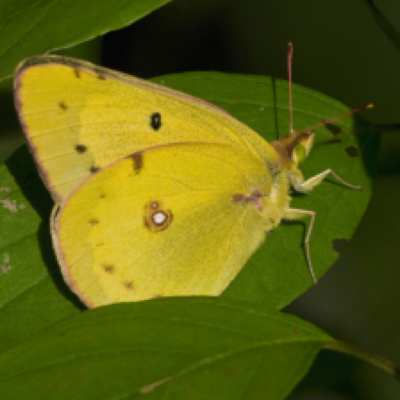
\includegraphics[width=\linewidth]{saliency_quality/image_0106_ILSVRC2012_val_00019900.JPEG/original_image.png}
    \end{minipage}\hspace{\colSpace}%
    \begin{minipage}[c]{\colB\linewidth}
        \centering
        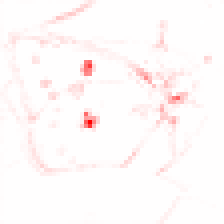
\includegraphics[width=\linewidth]{saliency_quality/image_0106_ILSVRC2012_val_00019900.JPEG/hybrid_lrp_scaling_max_winnerTakesItAllMaxpool_f10_cam_pp_abs.png}
    \end{minipage}\hspace{\colSpace}%
    \begin{minipage}[c]{\colB\linewidth}
        \centering
        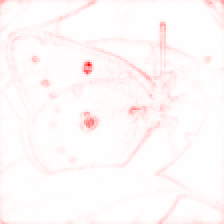
\includegraphics[width=\linewidth]{saliency_quality/image_0106_ILSVRC2012_val_00019900.JPEG/zennit_lrp_gamma0.25_features_5_abs.png}
    \end{minipage}\hspace{\colSpace}%
    \begin{minipage}[c]{\colB\linewidth}
        \centering
        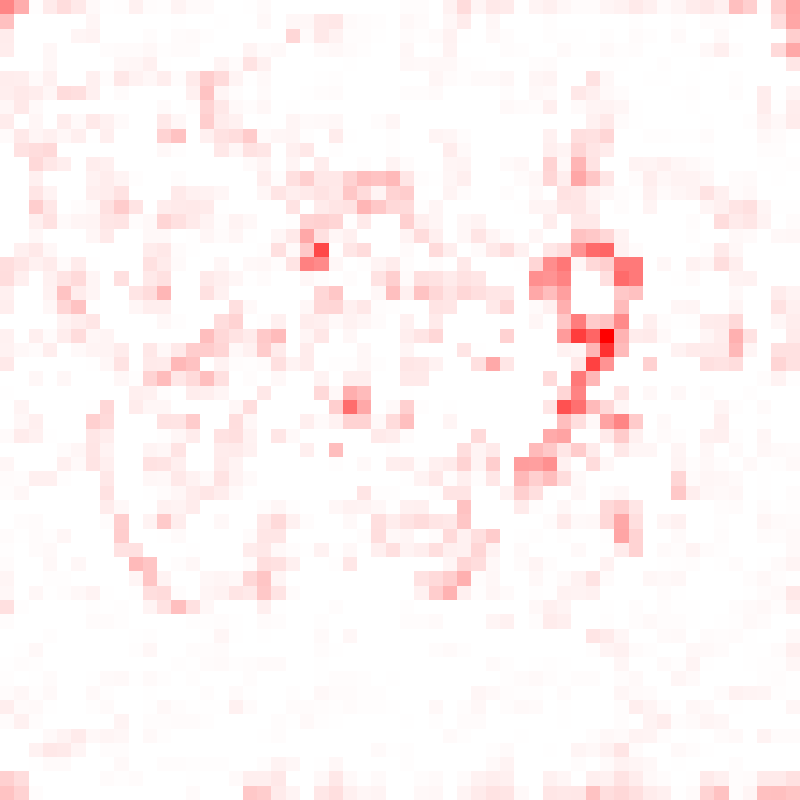
\includegraphics[width=\linewidth]{saliency_quality/image_0106_ILSVRC2012_val_00019900.JPEG/hybrid_cam_shift_40_scale_max_winnerTakesItAllMaxpool_f14_cam_g.png}
    \end{minipage}\hspace{\colSpace}%
    \begin{minipage}[c]{\colB\linewidth}
        \centering
        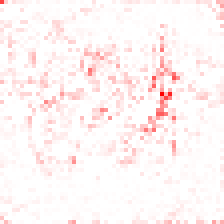
\includegraphics[width=\linewidth]{saliency_quality/image_0106_ILSVRC2012_val_00019900.JPEG/layer_cam_features_14_relu.png}
    \end{minipage}\hspace{\colSpace}%
    \begin{minipage}[c]{\colB\linewidth}
        \centering
        
\includegraphics[width=\linewidth]{saliency_quality/image_0106_ILSVRC2012_val_00019900.JPEG/hybrid_cam_shift_30_scale_max_winnerTakesItAllMaxpool_f26_cam_g_abs.png}
    \end{minipage}\hspace{\colSpace}%
    \begin{minipage}[c]{\colB\linewidth}
        \centering
        
\includegraphics[width=\linewidth]{saliency_quality/image_0106_ILSVRC2012_val_00019900.JPEG/layer_cam_features_26_relu.png}
    \end{minipage}\hspace{\colSpace}%
    \begin{minipage}[c]{\colB\linewidth}
        \centering
        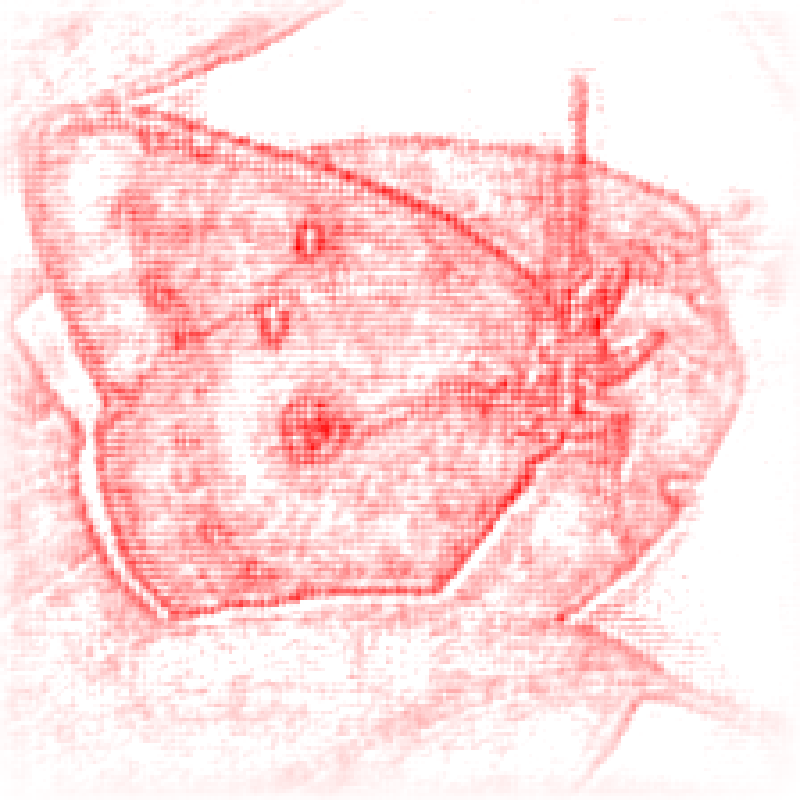
\includegraphics[width=\linewidth]{saliency_quality/image_0106_ILSVRC2012_val_00019900.JPEG/hybrid_grad_shift_30_max_winnerTakesItAllMaxpool_f0_grad_pp.png}
    \end{minipage}%

    \vspace{0.25cm}

    \begin{minipage}[c]{\colA\linewidth}
        \centering
        \small goldfish\\[1pt]
        {\scriptsize (1.0000)}
    \end{minipage}\hspace{\colSpace}%
    \begin{minipage}[c]{\colB\linewidth}
        \centering
        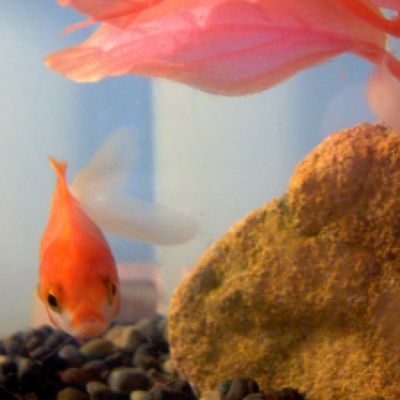
\includegraphics[width=\linewidth]{saliency_quality/image_0005_ILSVRC2012_val_00020785.JPEG/original_image.png}
    \end{minipage}\hspace{\colSpace}%
    \begin{minipage}[c]{\colB\linewidth}
        \centering
        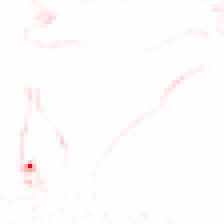
\includegraphics[width=\linewidth]{saliency_quality/image_0005_ILSVRC2012_val_00020785.JPEG/hybrid_lrp_scaling_max_winnerTakesItAllMaxpool_f10_cam_pp_abs.png}
    \end{minipage}\hspace{\colSpace}%
    \begin{minipage}[c]{\colB\linewidth}
        \centering
        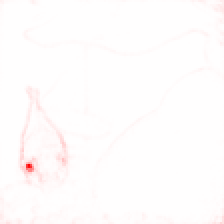
\includegraphics[width=\linewidth]{saliency_quality/image_0005_ILSVRC2012_val_00020785.JPEG/zennit_lrp_gamma0.25_features_5_abs.png}
    \end{minipage}\hspace{\colSpace}%
    \begin{minipage}[c]{\colB\linewidth}
        \centering
        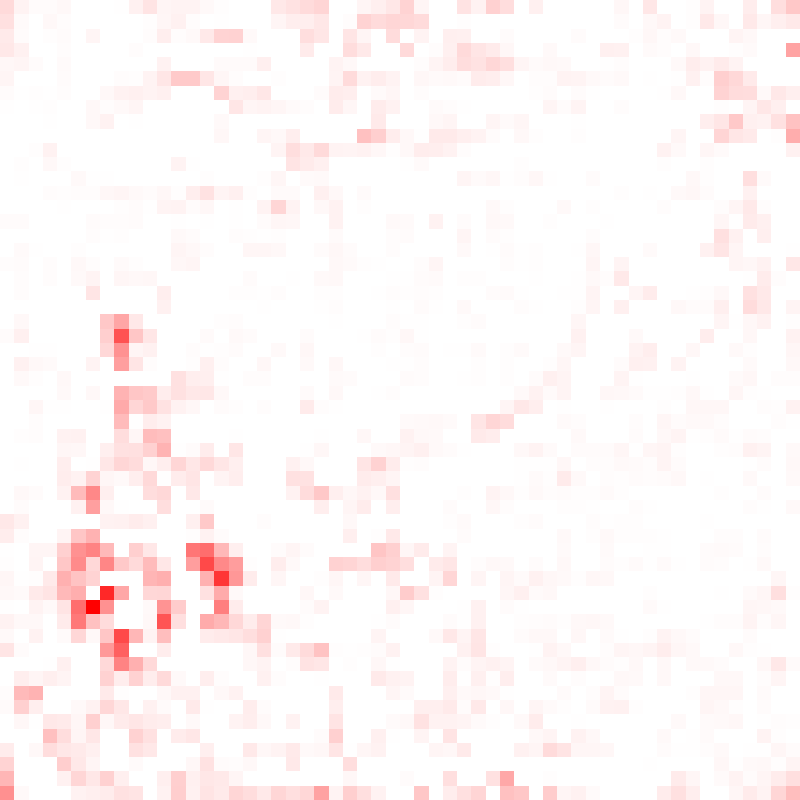
\includegraphics[width=\linewidth]{saliency_quality/image_0005_ILSVRC2012_val_00020785.JPEG/hybrid_cam_shift_40_scale_max_winnerTakesItAllMaxpool_f14_cam_g.png}
    \end{minipage}\hspace{\colSpace}%
    \begin{minipage}[c]{\colB\linewidth}
        \centering
        
\includegraphics[width=\linewidth]{saliency_quality/image_0005_ILSVRC2012_val_00020785.JPEG/layer_cam_features_14_relu.png}
    \end{minipage}\hspace{\colSpace}%
    \begin{minipage}[c]{\colB\linewidth}
        \centering
        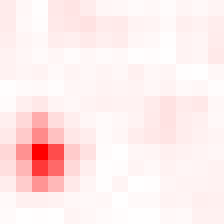
\includegraphics[width=\linewidth]{saliency_quality/image_0005_ILSVRC2012_val_00020785.JPEG/hybrid_cam_shift_30_scale_max_winnerTakesItAllMaxpool_f26_cam_g_abs.png}
    \end{minipage}\hspace{\colSpace}%
    \begin{minipage}[c]{\colB\linewidth}
        \centering
        
\includegraphics[width=\linewidth]{saliency_quality/image_0005_ILSVRC2012_val_00020785.JPEG/layer_cam_features_26_relu.png}
    \end{minipage}\hspace{\colSpace}%
    \begin{minipage}[c]{\colB\linewidth}
        \centering
        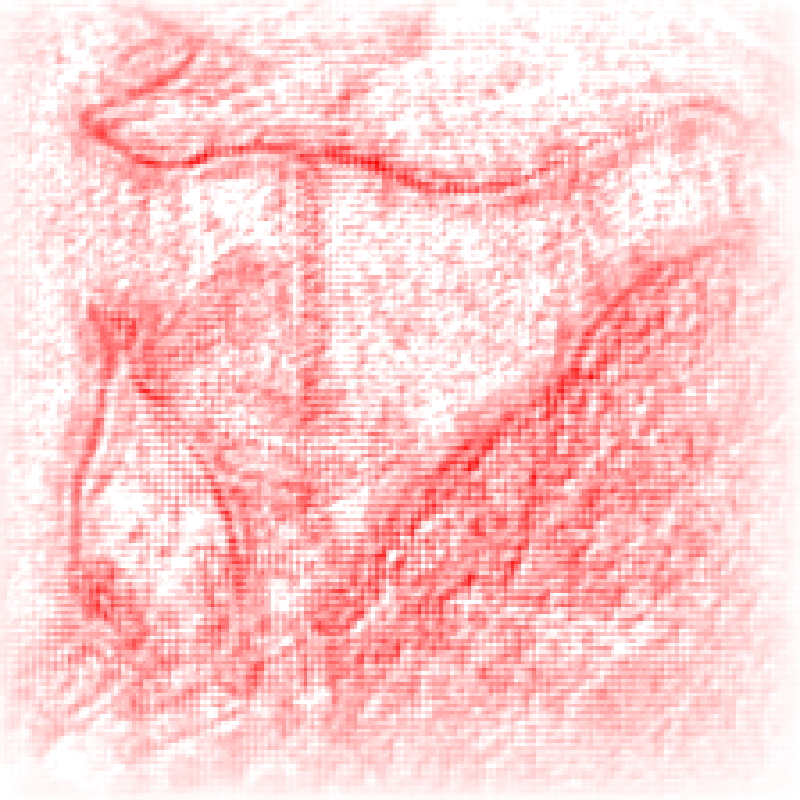
\includegraphics[width=\linewidth]{saliency_quality/image_0005_ILSVRC2012_val_00020785.JPEG/hybrid_grad_shift_30_max_winnerTakesItAllMaxpool_f0_grad_pp.png}
    \end{minipage}%

    \caption{Saliency map comparison for VGG16 on our custom ImageNet-S test split. Each row shows the predicted class (with confidence), original image, and saliency maps from different methods.}
    \label{fig:vgg_saliency_comparison_main}
\end{figure*}


\subsection{Evaluation Framework and Metrics} \label{subsec:eval_framework}

We evaluate explanations using the Quantus library \citep{Hedstrom2023}, which provides standardized implementations of XAI metrics across key desiderata including \emph{faithfulness}, \emph{localization} and \emph{robustness}.

We adopt Quantus recommended default settings with several modifications for computational efficiency and to match common XAI evaluation practices. Full configurations and seeds are included in the supplementary code.              

Faithfulness metrics, such as \emph{Pixel Flipping} \citep{Bach2015} and \emph{Selectivity} \citep{Montavon2018}, assess whether explanations reflect the model's true decision process. Pixel Flipping measures the drop of           
the respective class logit when input features are replaced in decreasing attribution order. The Quantus evaluator broadcasts the spatial attribution over color channels and perturbs 112 scalar features of the flattened $C\times H\times W$ input per step, replacing them with the input mean. For $3\times224\times224$ RGB inputs, this feature space has dimension $150{,}528$. We report the area under the curve (AUC) of the score drop at $5\%$ and $20\%$, where a faster drop means higher area under the drop curve. Selectivity replaces non-overlapping $8\times8$ spatial patches with the input mean, in decreasing order of summed attribution.
Here, by the Quantus standard implementation a smaller value indicates a faster drop.

Localization metrics evaluate whether explanations highlight the correct spatial regions. \emph{Attribution Localization} \citep{Kohlbrenner2020} computes the ratio of attribution mass within the ground-truth segmentation          
mask and the \emph{Pointing Game} \citep{Zhang2018pointinggame} checks whether the maximum-attribution pixel lies inside the segmentation mask.
We use the segmentation masks provided by ImageNet-S for both metrics.

Robustness metrics, such as \emph{Maximum Sensitivity} \citep{Yeh2019}, quantify the stability of explanations under perturbations, where lower values indicate more stable explanations. We compute this metric with 25 random             
samples per image.
For all metrics we disable Quantus to take the absolute value of the attribution maps 
except for Maximum Sensitivity.

\FloatBarrier

\paragraph{Automated Layer Selection}
For each split based attribution method and the baselines $\gamma$-LRP, standard LayerCAM, standard GradCAM, Guided Backpropagation and Guided LayerCAM we evaluate all layer–formula combinations on the validation set across all Quantus metrics.
This selection includes the layer-wise decision if to apply the absolute value to the attribution maps and layer-wise configurations for the split methods.
We select the configuration that (i) have the best average rank in the two considered localization metrics as well as (ii) the best average rank across the Pixel Flipping metrics.
Configurations are selected on the custom validation subset of ImageNet-S and evaluated on the custom test subset, keeping configuration selection separate from test measurement.

\subsection{Results}

\subsubsection{Qualitative Analysis}

\Cref{fig:vgg_saliency_comparison_main} qualitatively compares saliency maps from our split methods with their baseline counterparts at the best-performing layers.
Mid-layer SplitCAM shares key visual characteristics with classical $\gamma$-LRP from earlier layers.
Compared to standard LayerCAM on the same layer it focuses more weight to all object pixels, while still marking the key object features as especially important.
For $\alpha \ll 0.5$, SplitGrad yields less focused yet finely aligned gradients that closely follow image details. We attribute this to the Maxout activation retaining preactivation information, unlike ReLU, which discards it in inactive neurons. 
Overall, mid-layer SplitCAM offers an effective balance between interpretability and focus (low entropy).

\subsubsection{Quantitative Analysis}

\begin{table*}[htb!]
    \centering
    \small
    \caption{Comprehensive XAI Evaluation Results (ResNet18). The triples $x.y.z$ are a ResNet18 internal indexing of convolutional layer, at which the attribution maps are calculated. See the caption of \cref{tab:eval_res_main} for further abbreviations and table explanaition.}
    \label{tab:eval_res_main}
    \begin{tabular}{p{4cm}|cc|cccccc}
        \toprule
        \textbf{Method} & \textbf{Layer} & \textbf{Abs} & \textbf{Select.} & \textbf{Attr. Loc.} & \textbf{Point.} & \textbf{Pixel Fl. (AUC@5)} & \textbf{Pixel Fl. (AUC@20)} & \textbf{Max Sens.} \\
         & & & \textbf{$\downarrow$} & \textbf{$\uparrow$} & \textbf{$\uparrow$} & \textbf{$\uparrow$} & \textbf{$\uparrow$} & \textbf{$\downarrow$} \\
        
         \midrule
        \multicolumn{9}{c}{\textit{SplitCAM Methods}} \\
        \midrule
        SplitCAM (sc, $\alpha = 0.3$, wta) & (1.0.2, g) & n & \fboxsep=0.5pt\colorbox{red!20}{\textbf{3.503}} & 0.487 & 0.747 & 0.168 & 1.395 & 1.277 \\
        SplitCAM (sc, $\alpha = 0.3$, wta) & (4.1.2, g) & n & 5.654 & \fboxsep=0.5pt\colorbox{red!20}{\textbf{0.673}} & \fboxsep=0.5pt\colorbox{red!20}{\textbf{0.972}} & 0.081 & 0.880 & 0.233 \\
        SplitGrad ($\alpha = 0.3$, wta) & (1.0.2, g) & y & 4.449 & 0.513 & 0.777 & 0.149 & 1.266 & 0.813 \\
        SplitGrad ($\alpha = 0.3$, wta) & (4.1.2, g) & y & 5.663 & 0.649 & 0.972 & 0.082 & 0.882 & 0.219 \\
        SplitLRP (sc, wta) & (conv1, pos) & y & 6.313 & 0.506 & 0.587 & 0.056 & 0.697 & 0.755 \\
        \midrule
        \multicolumn{9}{c}{\textit{Baselines (With Layer Optimization)}} \\
        \midrule
        GradCAM & 4.1.2 & n & 6.070 & 0.554 & 0.945 & 0.076 & 0.829 & \fboxsep=0.5pt\colorbox{red!20}{\textbf{0.131}} \\
        LayerCAM & 2.0.2 & n & 3.690 & 0.549 & 0.865 & 0.144 & 1.428 & 0.913 \\
        LayerCAM & 4.1.1 & n & 5.661 & 0.664 & 0.971 & 0.083 & 0.890 & 0.227 \\
        LRP $\gamma=0.25$ & conv1 & y & 3.550 & 0.656 & 0.852 & \fboxsep=0.5pt\colorbox{red!20}{\textbf{0.213}} & 1.737 & 0.521 \\
        \midrule
        \multicolumn{9}{c}{\textit{Baselines}} \\
        \midrule
        Guided Backprop & conv1 & n & 3.517 & 0.621 & 0.867 & 0.212 & \fboxsep=0.5pt\colorbox{red!20}{\textbf{1.757}} & 0.459 \\
        Gradient SHAP & conv1 & y & 5.269 & 0.527 & 0.779 & 0.166 & 1.227 & 1.074 \\
        Integrated Gradients & conv1 & y & 5.265 & 0.528 & 0.777 & 0.167 & 1.226 & 0.994 \\
        Feature Ablation & conv1 & n & 4.655 & 0.136 & 0.684 & 0.188 & 1.388 & 1.077 \\
        Occlusion & conv1 & n & 5.300 & 0.179 & 0.726 & 0.130 & 1.030 & 0.785 \\
        Deconvolution & conv1 & n & 3.934 & 0.484 & 0.666 & 0.147 & 1.203 & 0.751 \\
        Random Baseline & - & y & 4.071 & 0.425 & 0.440 & 0.147 & 1.067 & -- \\
        \bottomrule
    \end{tabular}
\end{table*}
    

\Cref{tab:eval_vgg_main} and \cref{tab:eval_res_main} compare selected attribution configurations on VGG16 and ResNet18 across five key Quantus metrics: Selectivity, Attribution Localization, Pointing Game accuracy, Pixel Flipping (AUC@5 and AUC@20) and Maximum Sensitivity.
The \emph{Abs} column specifies whether absolute saliency values were used prior to evaluation in Quantus.
A full table and explanation of both VGG16 and ResNet18 evaluation results with all selected layers and other parameter configurations is found in \cref{app:saliency}.

Overall, the considered backpropagation-based attribution methods heavily depend on the selected network layer, also see \cref{app:ablation} for extensive ablation.

On VGG16, the gains depend on the metric and configuration. In \cref{tab:eval_vgg_main}, SplitCAM reaches a Pointing Game score of $0.938$ versus $0.887$ for Guided Backprop, Attribution Localization of $0.651$ versus $0.632$ for Guided Backprop, and Selectivity of $2.727$ versus $2.792$ for LayerCAM. These SplitCAM values come from different layers.
LayerCAM retains the highest Pixel Flipping score-drop AUCs, $0.317$ and $2.474$, compared with SplitCAM's $0.300$ and $2.404$ in the displayed configurations. SplitLRP has the lowest Maximum Sensitivity, $0.282$, compared with $0.375$ for Guided Backprop. Its Pointing Game score exceeds those of the displayed classical $\gamma$-LRP configurations, while its Attribution Localization and Pixel Flipping scores are lower.

On ResNet18, SplitCAM has the lowest reported Selectivity, $3.503$, compared with $3.517$ for the strongest baseline, Guided Backprop: a numerical difference of $0.014$. SplitCAM and SplitGrad reach a Pointing Game score of $0.972$, compared with LayerCAM's $0.971$. SplitCAM's Attribution Localization of $0.673$ exceeds LayerCAM's $0.664$, but the full comparison reports a higher value of $0.742$ for Guided Grad-CAM (\cref{tab:xai_eval_comprehensive_res}). The baselines also retain the best Pixel Flipping scores and Maximum Sensitivity, so the results support metric-specific gains.

\subsubsection{Ablation studies.} \label{subsec:ablation}


\begin{table}[h]
    \centering
    \footnotesize
    % \setlength{\tabcolsep}{1.5pt}
    % \renewcommand{\arraystretch}{1.0}
    %\renewcommand\cellalign{cc}

    \resizebox{1.0\columnwidth}{!}{%
    \begin{tabular}{|l|l|c|c|c|c|c|c|}
    \hhline{|-|-|------|}
    \textbf{Method} & \textbf{Metric} & $\alpha \ .50$ & $\alpha \ .45$ & $\alpha \ .40$ & $\alpha \ .35$ & $\alpha \ .30$ & $\alpha \ .00$ \\
    \hhline{|-|-|------|}
    \multirow{4}{*}{\makecell{\textbf{SplitGrad}\\(26, g)}} & Point. $\uparrow$ & 0.898 & 0.906 & 0.947 & \textbf{0.956} & 0.889 & 0.401 \\
    \hhline{|~|-|------|}
     & Attr. Loc. $\uparrow$ & 0.543 & 0.548 & 0.605 & \textbf{0.617} & 0.535 & 0.449 \\
    \hhline{|~|-|------|}
     & Max Sens. $\downarrow$ & 0.616 & 0.607 & 0.440 & 0.238 & 0.334 & \textbf{0.028} \\
    \hhline{|~|-|------|}
     & Pixel Fl. @20 $\uparrow$ & 1.527 & 1.534 & \textbf{1.581} & 1.448 & 1.317 & 1.247 \\
    \hhline{|-|-|------|}
    \multirow{4}{*}{\makecell{\textbf{SplitCAM}\\(26, +, g)}} & Point. $\uparrow$ & 0.868 & 0.868 & \textbf{0.938} & 0.933 & 0.613 & 0.855 \\
    \hhline{|~|-|------|}
     & Attr. Loc. $\uparrow$ & 0.550 & 0.554 & 0.635 & \textbf{0.663} & 0.403 & 0.513 \\
    \hhline{|~|-|------|}
     & Max Sens. $\downarrow$ & 0.691 & 0.682 & 0.457 & 0.265 & 0.251 & \textbf{0.120} \\
    \hhline{|~|-|------|}
     & Pixel Fl. @20 $\uparrow$ & 1.607 & \textbf{1.609} & 1.585 & 1.499 & 0.853 & 1.507 \\
    \hhline{|-|-|------|}
    \end{tabular}
    }%
    
    \caption{Comparison of different $\alpha$ parameters with two SplitGrad and SplitCAM base configurations, both in \emph{wta} and \emph{abs} mode.}
    \label{tab:alpha_ablation_main}
\end{table}

Table \ref{tab:alpha_ablation_main} presents the performance of two selected SplitGrad and SplitCAM configurations across different shifting parameters $\alpha$, evaluated on our custom ImageNet-S test split.
As explained in \cref{sec:backward} the $\alpha$ value determines how much we stablize the backward pass, where $\alpha=0$ results in no stabilization and $\alpha = 0.5$ results in local sensitivities resembling scaled versions of the original network gradient.
Within this ablation, reducing $\alpha$ from $0.5$ to $0.4$ improves Pointing Game and Attribution Localization for both configurations, while SplitCAM's Pixel Flipping AUC@20 decreases from $1.607$ to $1.585$. SplitGrad reaches its highest AUC@20 at $\alpha = 0.4$ and its highest localization scores at $\alpha = 0.35$; SplitCAM's Pointing Game and Attribution Localization optima occur at $0.4$ and $0.35$, respectively. Maximum Sensitivity is lowest at $\alpha = 0$ for both configurations. The sweep therefore supports a metric-dependent choice of $\alpha$ and does not isolate the effect of numerical stabilization from the change in attribution rule.
We provide further ablation studies in \cref{app:ablation}.
